\section{Identifying The Performance Gap Under Partial Observability}
\label{sec:po-identification}

The central question of this section is whether the performance collapse observed under partial observability is genuinely caused by information loss, or whether it reflects a deeper weakness in the rule-based controller itself. This identification step is necessary before any claim about memory can be grounded: if \task{NoMemory} were simply a weaker policy, then adding memory would be compensating for policy capacity rather than for observability.

\subsection{Full-Observable Identification Experiment}

\begin{figure}[t]
  \centering
  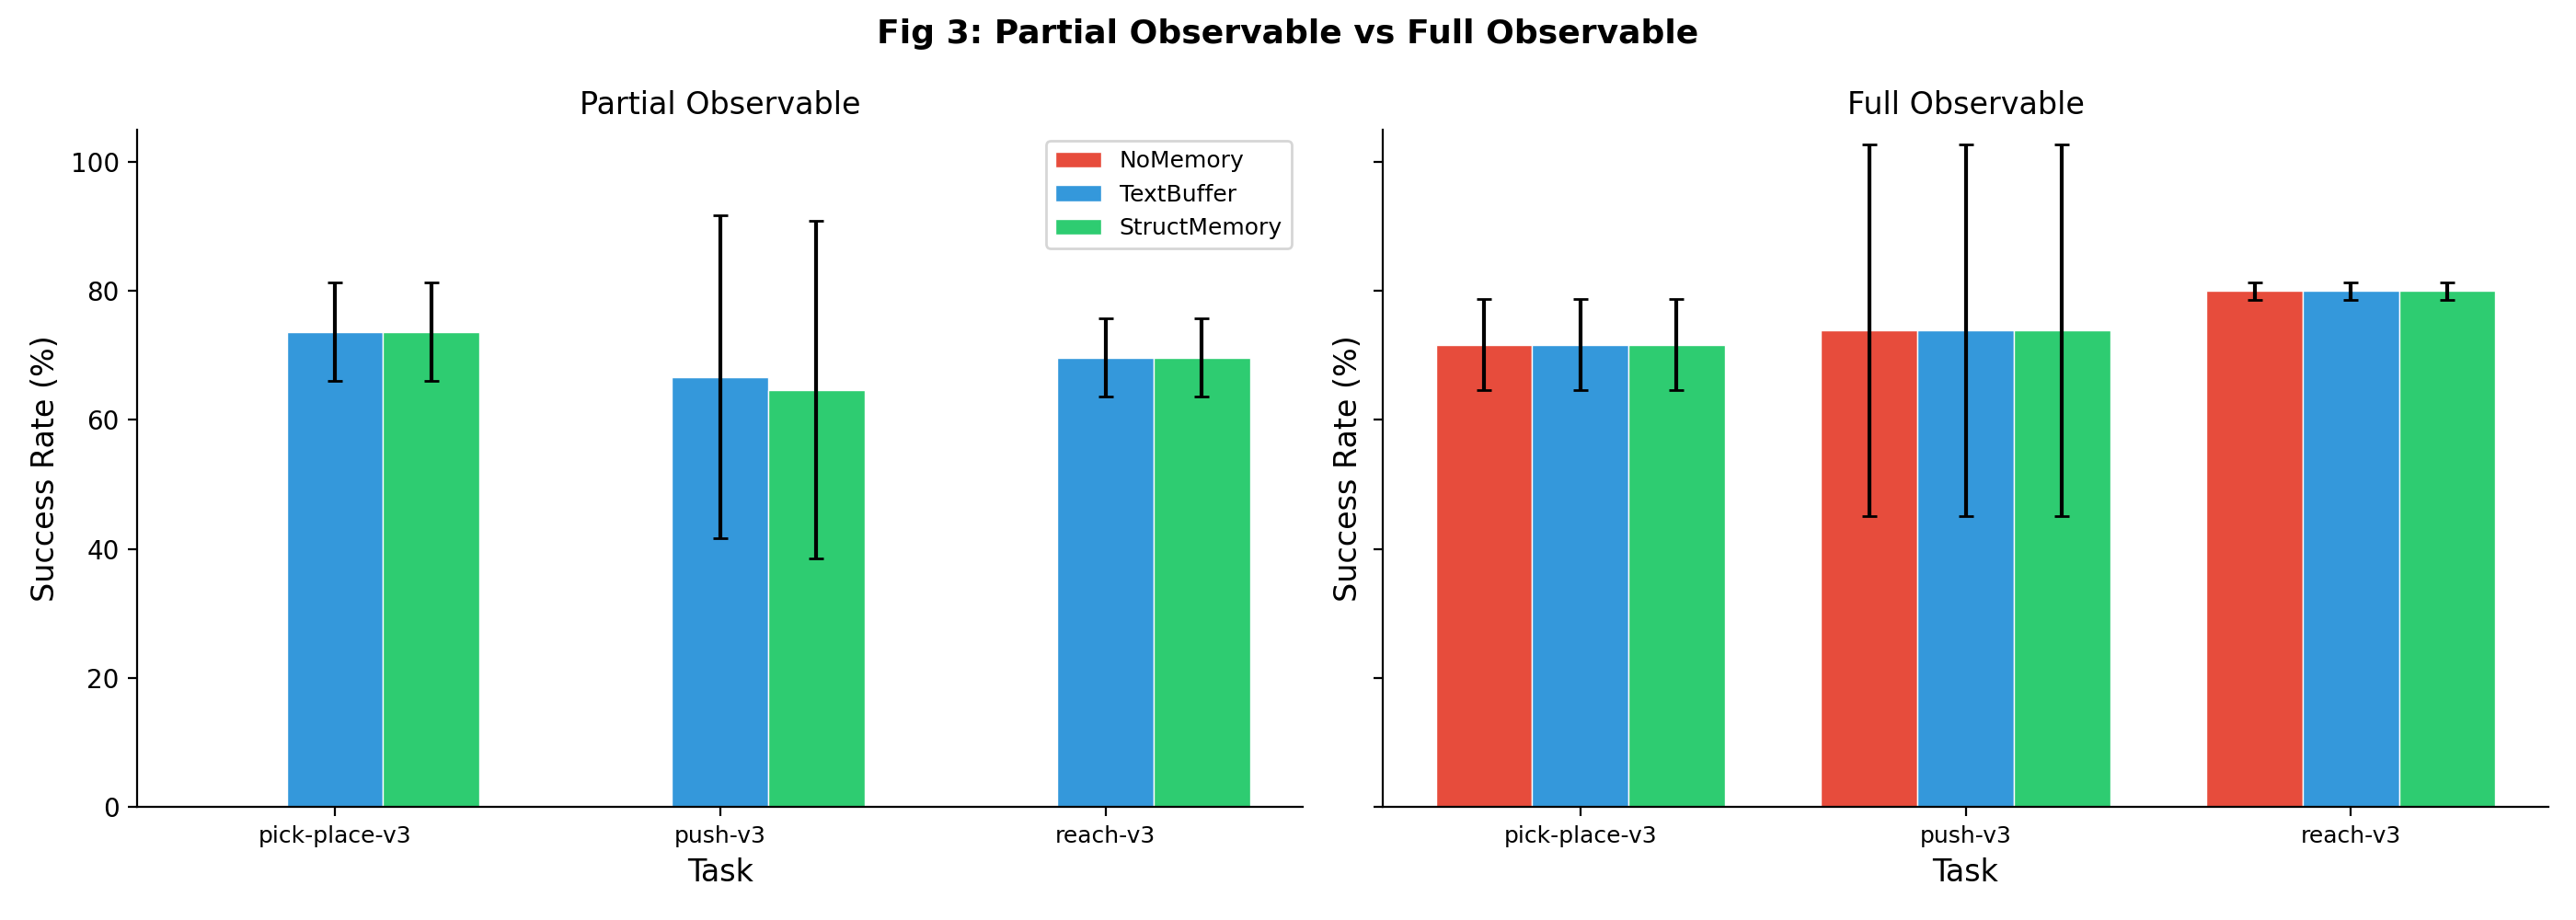
\includegraphics[width=0.92\linewidth]{figures/fig3_po_vs_fullobs.png}
  \caption{Partial-observability vs.\ full-observable comparison. Under FO, the gap between \task{NoMemory} and memory-enabled variants disappears on all solvable tasks, confirming that the PO gap is induced by information loss rather than policy incapacity.}
  \label{fig:fo-control}
\end{figure}

The FO control directly tests whether the PO gap reflects a memory requirement rather than a deeper weakness in the rule-based policy itself. As shown in Figure~\ref{fig:fo-control}, under full observability (3 seeds, 60 episodes per seed), all three policies converge on the three solvable tasks: \task{reach-v3} at $80.0 \pm 1.4\%$, \task{push-v3} at $73.9 \pm 28.7\%$, and \task{pick-place-v3} at $71.7 \pm 7.1\%$.

This result is central to the paper's interpretation. If \task{NoMemory} had remained far below the memory-enabled policies under FO, the PO explanation would have been incomplete---the gap would have reflected a general policy weakness rather than an observability effect. Instead, the FO result supports a narrower and stronger identification: in the current setup, the performance difference is primarily induced by partial observability rather than by a general incapacity of the rule-based controller.

\textbf{Note on experimental scale.} The FO control uses 3 seeds versus 5 seeds for the PO main experiment. The reported FO standard deviations are therefore wider in expectation and should not be compared directly to the PO values. Readers should treat the FO result as a directional identification check rather than a precision measurement.
\FloatBarrier

\subsection{Performance Under Partial Observability}

\begin{figure}[t]
  \centering
  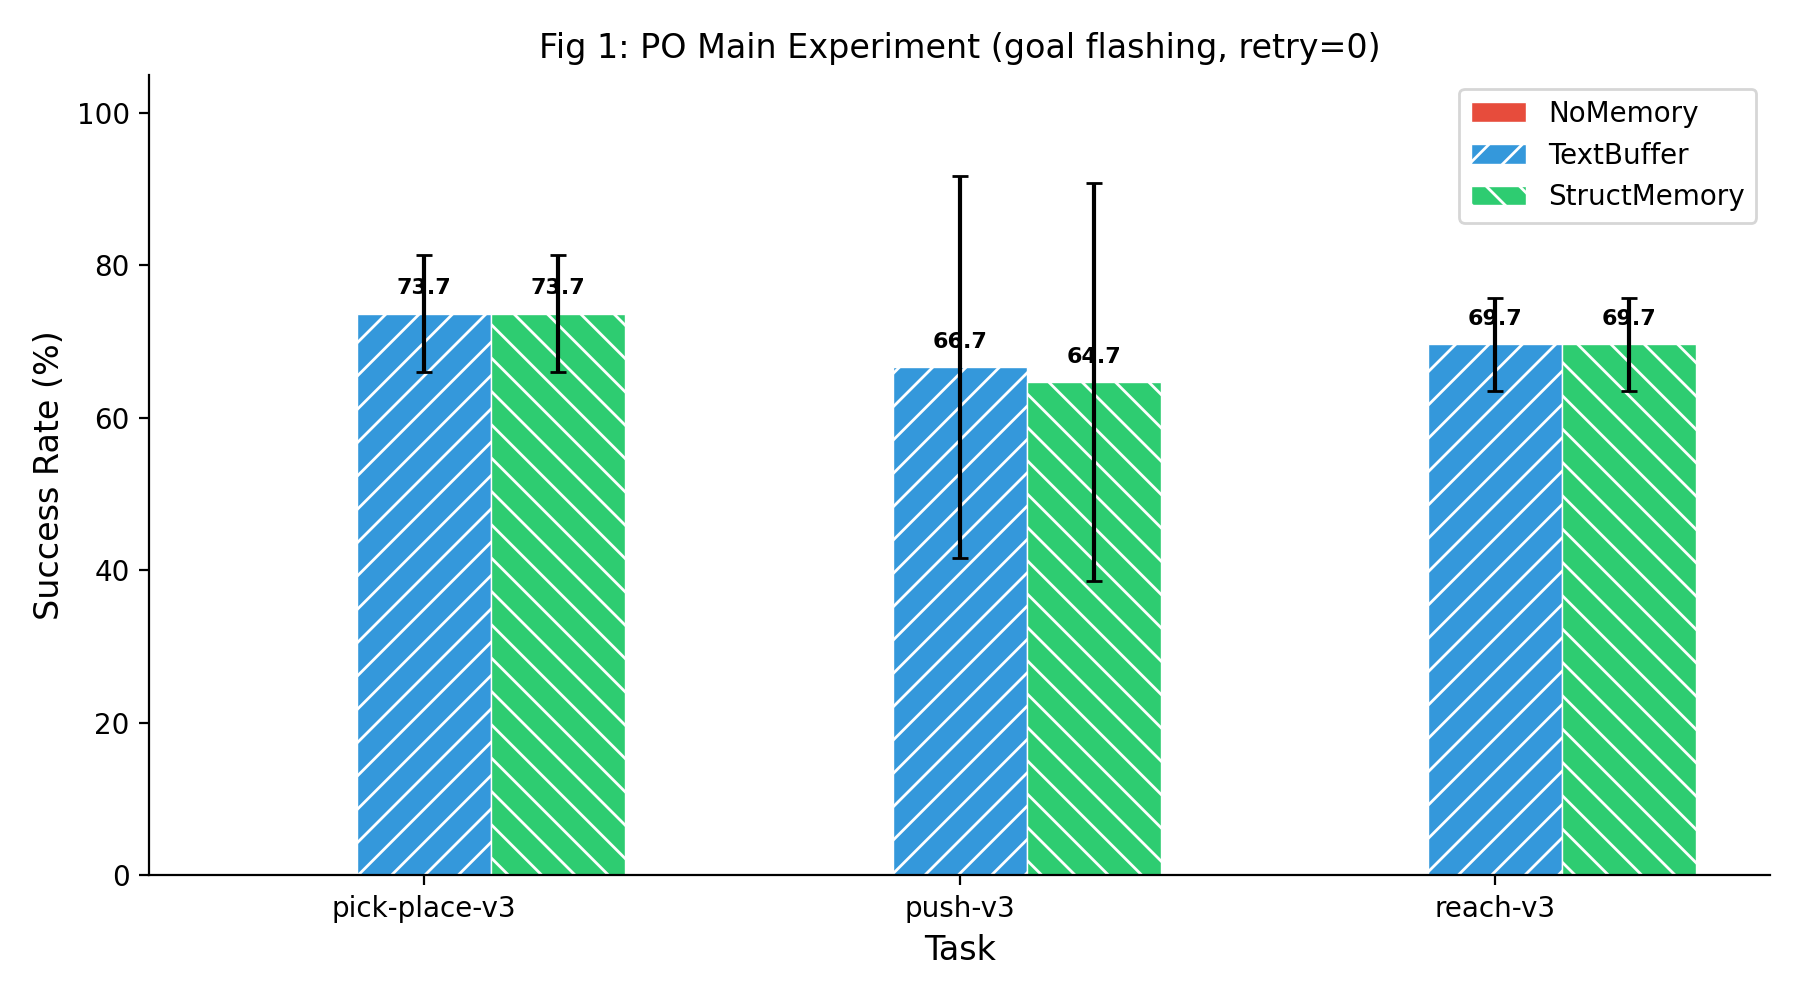
\includegraphics[width=0.92\linewidth]{figures/fig1_po_main_success_rate.png}
  \caption{Success rates under partial observability (\texttt{retry=0}). \task{NoMemory} collapses to 0\% on all tasks; memory-enabled variants recover substantial performance on three of four tasks.}
  \label{fig:po-main}
\end{figure}

\begin{table}[t]
\centering
\caption{Success rates (\%) on 9 MetaWorld tasks under Full-Observable (FO) and WeakPO conditions (\texttt{flash\_every}$=$20). Entries are mean $\pm$ std over 5 seeds $\times$ 60 episodes. \textbf{NM} = NoMemory, \textbf{TB} = TextBuffer, \textbf{SM} = StructMemory. $\dagger$ marks V1 FSM tasks; all others use V2 Goal-Relative FSM. $^{**}$ marks $p < 0.01$ for NM FO vs.\ WeakPO.}
\label{tab:main_results}
\resizebox{\textwidth}{!}{%
\begin{tabular}{l ccc c ccc c c}
\toprule
& \multicolumn{3}{c}{FO} & & \multicolumn{3}{c}{WeakPO} & & \\
\cmidrule(lr){2-4} \cmidrule(lr){6-8}
Task & NM & TB & SM & & NM & TB & SM & & NM $\Delta$(WeakPO$-$FO) \\
\midrule
\multicolumn{10}{l}{\textit{Core Tasks (V1 FSM)$^\dagger$}} \\
Reach$^{**}$        & 82.3$\pm$9.5 & 82.3$\pm$9.5 & 82.3$\pm$9.5 & & 0.0$\pm$0.0 & 64.7$\pm$7.8 & 64.7$\pm$7.8 & & $-$82.3 \\
Push$^{**}$         & 64.3$\pm$29.7 & 66.0$\pm$28.5 & 64.3$\pm$29.7 & & 0.0$\pm$0.0 & 65.7$\pm$26.7 & 64.3$\pm$28.0 & & $-$64.3 \\
Pick-Place$^{**}$   & 74.0$\pm$7.1 & 74.0$\pm$7.1 & 74.0$\pm$7.1 & & 0.0$\pm$0.0 & 74.7$\pm$5.5 & 74.7$\pm$5.5 & & $-$74.0 \\
\midrule
\multicolumn{10}{l}{\textit{Extended Tasks (V2 Goal-Relative FSM)}} \\
Door-Open$^{**}$    & 90.3$\pm$5.7 & 91.0$\pm$5.1 & 90.3$\pm$5.7 & & 0.0$\pm$0.0 & 90.7$\pm$5.6 & 90.7$\pm$5.2 & & $-$90.3 \\
Drawer-Open$^{**}$  & 100.0$\pm$0.0 & 100.0$\pm$0.0 & 100.0$\pm$0.0 & & 0.0$\pm$0.0 & 100.0$\pm$0.0 & 100.0$\pm$0.0 & & $-$100.0 \\
Faucet-Open$^{**}$  & 56.3$\pm$5.6 & 54.0$\pm$3.8 & 56.3$\pm$5.6 & & 2.3$\pm$2.2 & 54.0$\pm$3.8 & 56.0$\pm$4.9 & & $-$54.0 \\
Button-Press        & 60.3$\pm$13.2 & 59.7$\pm$15.2 & 60.3$\pm$13.2 & & 61.3$\pm$13.9 & 60.7$\pm$13.3 & 58.7$\pm$15.2 & & $+$1.0 \\
Sweep$^{**}$        & 52.0$\pm$3.0 & 52.0$\pm$3.2 & 52.0$\pm$3.0 & & 0.0$\pm$0.0 & 51.0$\pm$3.2 & 51.7$\pm$2.4 & & $-$52.0 \\
Shelf-Place$^{**}$  & 89.0$\pm$6.3 & 84.7$\pm$5.2 & 89.0$\pm$6.3 & & 0.0$\pm$0.0 & 84.7$\pm$5.1 & 89.0$\pm$6.3 & & $-$89.0 \\
\bottomrule
\end{tabular}%
}
\end{table}


With the FO identification in place, we now report the main PO results. As shown in Table~\ref{tab:main-results} and Figure~\ref{fig:po-main}, under the PO protocol with \texttt{retry=0}, \task{NoMemory} achieves $0.0 \pm 0.0$ success on all four tasks. The memory-enabled variants recover non-trivial performance on three tasks: \task{reach-v3} reaches $69.7 \pm 6.1\%$ for both \task{TextBuffer} and \task{StructMemory}, \task{push-v3} reaches $66.7 \pm 25.1\%$ and $64.7 \pm 26.1\%$, and \task{pick-place-v3} reaches $73.7 \pm 7.6\%$ for both. \task{door-open-v3} remains at $0.0\%$ for all policies.

An important detail is variance: \task{push-v3} exhibits high across-seed variability (std $\approx$ 25--26 percentage points), indicating sensitivity to initialization and execution noise even in the solved regime. We hypothesize that two factors drive this instability: (1) the initial object position sampled at reset spans a wide spatial range, causing the approach trajectory length to vary substantially across seeds; and (2) the PD controller's fixed gains interact inconsistently with surface friction when the push contact angle deviates from nominal---a regime where small perturbations can redirect the object away from the goal. We return to this point in the Limitations section.

\subsection{PO Severity Gradient: The Memory Necessity Curve}

\begin{figure}[t]
  \centering
  \includegraphics[width=0.92\linewidth]{figures/fig_flash_every_necessity_curve_5seeds.pdf}
  \caption{Memory Necessity Curve: success rate as a function of goal-observation interval (\texttt{flash\_every}). \task{NoMemory} partially functions when the goal is flashed every 5 steps but collapses at $\geq$10. Memory-enabled variants remain stable across all intervals.}
  \label{fig:flash-every}
\end{figure}

\input{tables/table4_flash_every}
\FloatBarrier

The PO/FO comparison establishes that the gap is caused by observability loss, but it does not reveal whether memory necessity is a binary property or a graded one. The flash-every ablation addresses this question by varying the severity of partial observability. Table~\ref{tab:flash-every} reports the \emph{NoMemory} column to highlight the collapse threshold; the stability of \task{TextBuffer} and \task{StructMemory} across flash intervals is visualized in Figure~\ref{fig:flash-every}.

As shown in Figure~\ref{fig:flash-every} and Table~\ref{tab:flash-every}, \task{NoMemory} exhibits a sharp threshold on \task{reach-v3} and \task{push-v3}. When the goal is flashed every 5 steps, \task{NoMemory} achieves $38.7\%$ on \task{reach-v3} and $41.7\%$ on \task{push-v3}---partial but non-trivial performance. When the flash interval increases to 10 steps, \task{NoMemory} drops to $4.0\%$ on \task{reach-v3} and $10.7\%$ on \task{push-v3}. At flash intervals of 20 or above, \task{NoMemory} collapses to $0\%$ on all tasks. On \task{pick-place-v3}, \task{NoMemory} remains at $0\%$ even at flash=5, indicating that the multi-stage grasp sequence makes this task strictly memory-dependent regardless of observation frequency. In contrast, both \task{TextBuffer} and \task{StructMemory} maintain stable performance ($57$--$75\%$) across all flash frequencies on all three tasks.

This curve reveals that memory necessity is not a binary property but depends on PO severity. Below a critical observation frequency, the memory-free controller can partially function by relying on recent goal information; above that threshold, persistent memory becomes a necessary condition for non-trivial performance.

\subsection{Goal-Relative Control and Contact-Rich Task Extension}
\label{sec:contact-rich}

The original task suite (reach, push, pick-place) involves non-contact or simple contact dynamics. To test whether the PO/memory finding extends to contact-rich manipulation, we introduce a \emph{Goal-Relative} control architecture and evaluate it on six additional MetaWorld tasks: \task{door-open-v3}, \task{drawer-open-v3}, \task{faucet-open-v3}, \task{button-press-topdown-v3}, \task{sweep-v3}, and \task{shelf-place-v3}.

\textbf{Goal-Relative architecture.}
In the original FSM, goal-oriented stages (e.g., push toward goal, move to shelf) read the goal position at build time and cache it. This design leaks goal information under PO: even when the goal is masked, the cached value remains available, eliminating the FO/PO gap. The Goal-Relative architecture modifies every goal-oriented stage to read \texttt{obs.goal\_pos} at \emph{every} step. When the goal is not visible (i.e., \texttt{obs.goal\_pos} is zero), the stage returns a zero action (stop), making the controller's execution genuinely dependent on goal observability. This architectural change is necessary to create a meaningful PO condition for contact-rich tasks.

\input{tables/table2_contact_rich}

\begin{table}[t]
\centering
\caption{Goal-dependency gradient: FO--PO gap correlates with the fraction of FSM stages that require goal information. \emph{Goal-dependent stages} are those whose action direction or target position is computed from \texttt{obs.goal\_pos} at every step. \emph{Gap} is the NoMemory FO--PO difference in percentage points.}
\label{tab:goal-dependency}
\begin{tabular}{@{}lccc@{}}
\toprule
Task & Goal-dep.\ stages & Total stages & FO--PO Gap \\
\midrule
drawer-open-v3 & 1 (pull) & 4 & +100 \\
door-open-v3 & 1 (pull) & 4 & +90 \\
shelf-place-v3 & 2 (move, descend) & 7 & +89 \\
faucet-open-v3 & 1 (turn) & 4 & +54 \\
sweep-v3 & 3 (approach, descend, push) & 4 & +52 \\
button-press-v3 & 0 (press is fixed down) & 3 & $-$1 \\
\bottomrule
\end{tabular}
\end{table}

Table~\ref{tab:contact-rich} reports the full FO/PO matrix (5 seeds, 60 episodes per seed) for the six contact-rich tasks. The results reveal a clear \emph{goal-dependency gradient}:

\begin{itemize}
\item \textbf{Strong goal-dependency} (gap $\geq$ 89pp): \task{drawer-open-v3} (+100pp), \task{door-open-v3} (+90pp), and \task{shelf-place-v3} (+89pp). In these tasks, the critical manipulation stage---pulling a handle, moving an object to a shelf---requires the goal position to determine the action direction. Without the goal, \task{NoMemory} cannot compute a meaningful action and stops.

\item \textbf{Moderate goal-dependency} (gap 52--54pp): \task{faucet-open-v3} (+54pp) and \task{sweep-v3} (+52pp). These tasks have goal-dependent stages, but the action has a stronger prior component (e.g., the faucet turn direction has a dominant rotational component; the sweep push has a dominant forward component), reducing the marginal contribution of goal information.

\item \textbf{Weak goal-dependency} (gap $\approx$ 0pp): \task{button-press-topdown-v3} ($-$1pp). The press stage is a fixed downward force; the goal only provides a minor xy correction. Removing goal information has negligible effect on the action.
\end{itemize}

Table~\ref{tab:goal-dependency} makes this gradient explicit by annotating each task's FSM stages. The FO--PO gap is not random---it directly reflects the degree to which the task's manipulation stages depend on goal information. Notably, \task{sweep-v3} has the highest fraction of goal-dependent stages (3/4) yet a moderate gap (+52pp), suggesting that the gap magnitude depends on both the \emph{fraction} and the \emph{marginal contribution} of goal information within each stage.

Across all five high-gap tasks, both \task{TextBuffer} and \task{StructMemory} recover to within 1pp of their FO performance under PO, confirming that the memory mechanism is sufficient to bridge the goal-observability gap regardless of task dynamics.

Taken together, the FO identification experiment, the PO main table, the Memory Necessity Curve, and the contact-rich extension support a specific controlled reading: the performance gap under the current PO protocol primarily corresponds to information loss rather than to a general incapacity of the rule-based controller. Furthermore, the magnitude of the gap tracks the task's goal-dependency structure---a finding that extends the PO/memory relationship beyond the original three tasks. This reading grounds the subsequent sections, which examine what kind of memory matters and how the bottleneck shifts as task complexity increases.
